% Länge 1:
% Länge 2:
% normale Schwingung:
% Exp L1:   T_linkes_L1: 1.237+/-0.005 in s       T_rechtes_L1: 1.238+/-0.004in s
% Exp L1 :  T_linkes_L2: 1.602+/-0.006 in s       T_rechtes_L2: 1.608+/-0.006in s
% gleichsinnige Schwingung:
% Exp L1:   T_gleich_L1: 1.194+/-0.004 in s       omega_gleich_L1: 5.261+/-0.017 in 1/s
% Exp L2:   T_gleich_L2: 1.567+/-0.010 in s       omega_gleich_L2: 4.009+/-0.025 in 1/s
% gegensinnige Schwingung
% Exp L1:   T_gegen_L1: 1.031+/-0.008 in s        omega_gegen_L1: 6.09+/-0.05 in 1/s
% Exp L2:   T_gegen_L2: 1.420+/-0.006 in s        omega_gegen_L2: 4.426+/-0.017 in 1/s
% Kopplungskonstanten:
% Kopplungskonstante K_L1:    0.146+/-0.008
% Kopplungskonstante K_L2:    0.099+/-0.007
% Gekoppelte Schwingung
% Exp L1:   T_schwingung_L1: 1.10+/-0.04 in s     Exp?????: omega_schwingung_L1: 5.72+/-0.20 in 1/s
% Exp L1:   T_schwebung_L1: 7.119+/-0.009 in s    omega_schwebung_L1: -0.83+/-0.05 in 1/s
% Exp L2:   T_schwingung_L2: 1.546+/-0.011 in s   Exp?????: omega_schwingung_L2: 4.065+/-0.030 in 1/s
% Exp L2:   T_schwebung_L2: 15.741+/-0.013 in s   omega_schwebung_L2: -0.417+/-0.030 in 1/s
\section{Auswertung}
\label{sec:Auswertung}

\begin{figure}
  \centering
  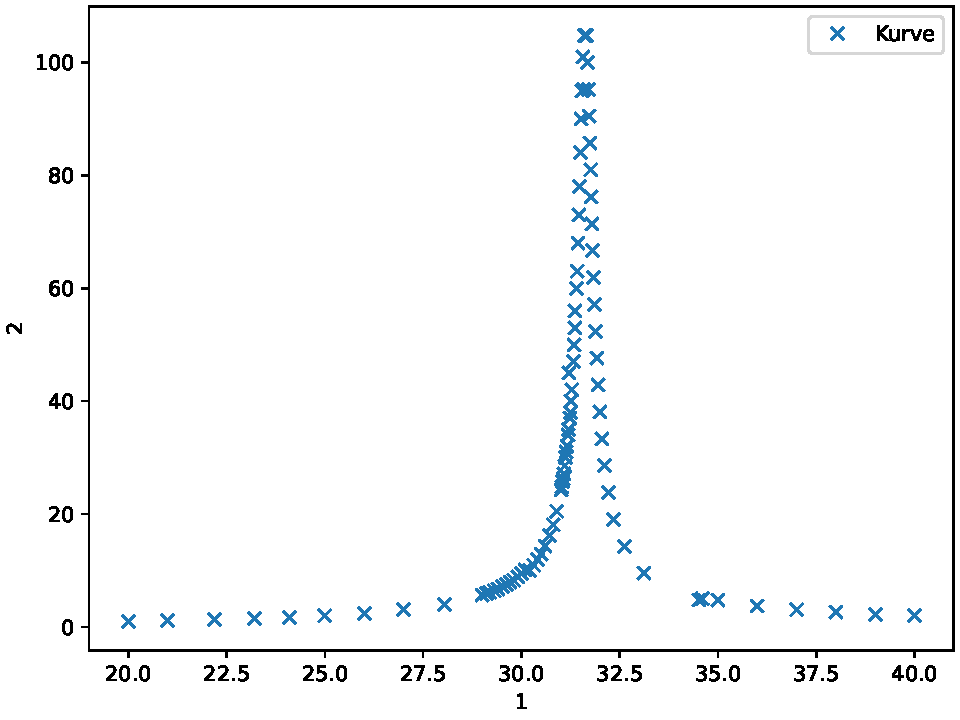
\includegraphics{plot.pdf}
  \caption{Plot.}
  \label{fig:plot}
\end{figure}

%Siehe \autoref{fig:plot}!